\chapter{Подготовка компонентов} \label{chap:altium-components}

Придётся принять реальность: чтобы сделать печатную плату, нужно знать размеры всех входящих в неё компонентов. Так что эта глава будет посвящена подготовке посадочных мест. 
Все стандартные компоненты будем брать из библиотеки \href{https://github.com/dee3mon/StudentsLibraryGIT}{StudentLibraryGit}, посадочные места более уникальных компонентов будем составлять самостоятельно. 

Почти все посадочные места создавались при помощи IPC Compliant Wizard, с внесением небольших правок; рисование УГО также тривиально, так что дальнейшее описание бужет в формате Посадочное место-3D модель (УГО можно будет увидеть в следующей главе).

\section{МШУ}

\begin{figure}[H]
	\centering

	\begin{subfigure}[b]{0.45\textwidth}
		\centering
		\includegraphics[width=0.6\textwidth, angle=-90]{LNA_PCB_View.pdf}
		\caption{}%
		\label{fig:LNA_PCB_View}
	\end{subfigure}
	\hfill
	\begin{subfigure}[b]{0.45\textwidth}
		\centering
		\includegraphics[width=\textwidth]{LNA_3D_View.png}
		\caption{}%
		\label{fig:LNA_3D_View}
	\end{subfigure}
	\caption{%
		Графика МШУ
		(а) Посадочное место;
		(б) 3D модель
	}%
	\label{fig:LNA_footprint}
\end{figure}

\section{Детектор мощности}

\begin{figure}[H]
	\centering
	\begin{subfigure}[b]{0.45\textwidth}
		\centering
		\includegraphics[width=0.55\textwidth, angle=-90]{PD_PCB_View.pdf}
		\caption{}%
		\label{fig:PD_PCB_View}
	\end{subfigure}
	\hfill
	\begin{subfigure}[b]{0.45\textwidth}
		\centering
		\includegraphics[width=0.9\textwidth]{PD_3D_View.png}
		\caption{}%
		\label{fig:PD_3D_View}
	\end{subfigure}
	\caption{%
		Графика ДМ
		(а) Посадочное место;
		(б) 3D модель
	}%
	\label{fig:PD_footprint}
\end{figure}

\section{Микроконтроллер}

Для приёма данных с детектора мощности и передачи их на внешнее устройство будем использовать PIC12F1822-I в корпусе SO-8. В него входит 10-битный АЦП с рабочим диапазоном Земля$\div$Опорное напряжение. Так как диапазон входных значений лежит от 0 до 1.2В, опорным напряжением будет 1.5~В. Данные с МК можно передавать по USART, SPI и I2C.


\begin{figure}[H]
	\centering
	\begin{subfigure}[b]{0.45\textwidth}
		\centering
		\includegraphics[width=\textwidth]{MC_PCB_View.pdf}
		\caption{}%
		\label{fig:MC_PCB_View}
	\end{subfigure}
	\hfill
	\begin{subfigure}[b]{0.45\textwidth}
		\centering
		\includegraphics[width=0.9\textwidth]{MC_3D_View.png}
		\caption{}%
		\label{fig:MC_3D_View}
	\end{subfigure}
	\caption{%
		Графика МК
		(а) Посадочное место;
		(б) 3D модель
	}%
	\label{fig:MC_footprint}
\end{figure}

\section{Питание}

Исходя из требований выбранных элементов, выбираем источник и стабилизаторы напряжения. Я положил глаз на линейный стабилизатор \href{https://www.analog.com/ru/products/lt1763.html}{LT1763}. Он имеет несколько моделей, в том числе и требуемые на 1.5~В, 2.5~В и 3.3~В с диапазоном входных значений до 20~В.

\begin{figure}[H]
	\centering\
	\begin{subfigure}[b]{0.45\textwidth}
		\centering
		\includegraphics[width=0.5\textwidth, angle=-90]{PM_PCB_View.pdf}
		\caption{}%
		\label{fig:PM_PCB_View}
	\end{subfigure}
	\hfill
	\begin{subfigure}[b]{0.45\textwidth}
		\centering
		\includegraphics[width=0.65\textwidth]{PM_3D_View.png}
		\caption{}%
		\label{fig:PM_3D_View}
	\end{subfigure}
	\caption{%
		Графика стабилизатора напряжения
		(а) Посадочное место;
		(б) 3D модель
	}%
	\label{fig:PM_footprint}
\end{figure}

\section{Микрополосковые элементы}
\begin{enumerate}
	\item Экспортируем МПЛ линии согласования, делитель мощности и фильтр из ADS через .dxf файлы; 
	\item Импортируем получившиеся конутры на слой top layer с толщиной линий в 0.1 мм;
	\item Удалим лишние внутренние контуры;
	\item Выделим замкнутые области и по команде Convert --- Create Region from Selected Primitives создадим залитые области;
	\item С помощью фильтра селекции удалим оставшиеся контура;
	\item Добавим пады по центру входов-выходов полосков.
\end{enumerate}
Пример импортированного микрополоскового компонента можно увидеть на Рис. \ref{fig:CL_Coupler_PCB}.
\begin{figure}[H]
	\centering
	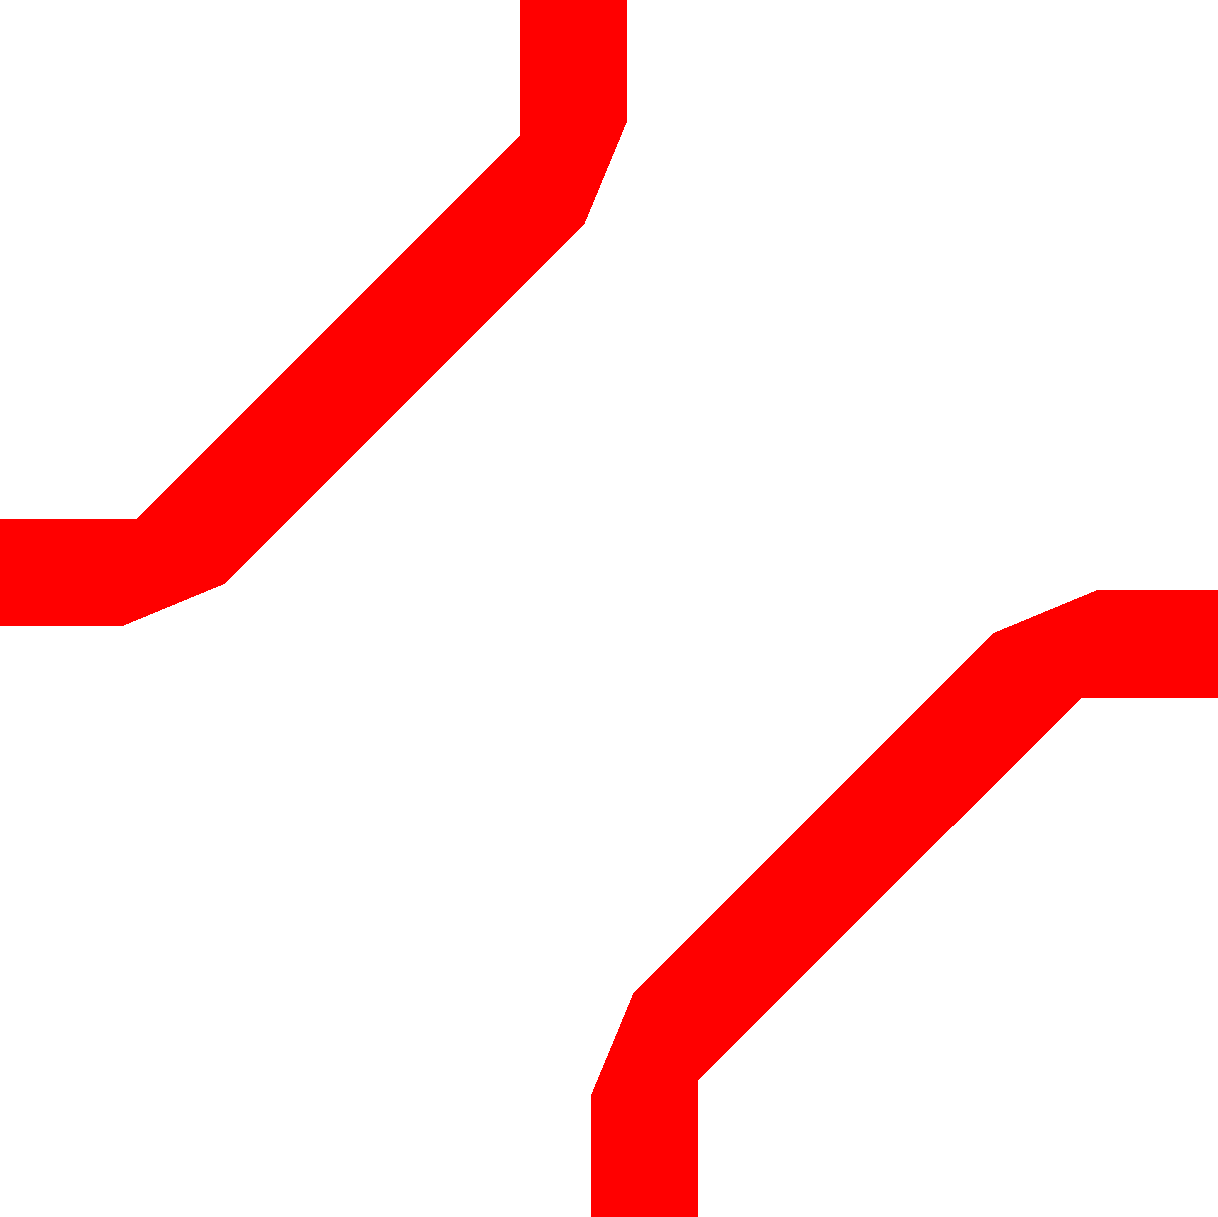
\includegraphics[width=0.9\textwidth, height=0.25\textheight, keepaspectratio]{CL_Coupler_PCB.pdf}
	\caption{Пример импортированной топологии.}%
	\label{fig:CL_Coupler_PCB}
\end{figure}
